%% This is a skeleton file demonstrating the use of IEEEtran.cls (requires IEEEtran.cls version 1.8a or later) with an IEEE conference paper.
%%
%% Modified by Khan Reaz( kahn.reaz@ieee.org)
%% Support sites:
%% http://www.ieee.org/

%%***********************************************************
%% Legal Notice:
%% This code is offered as-is without any warranty either expressed or implied; without even the implied warranty of MERCHANTABILITY or FITNESS FOR A PARTICULAR PURPOSE!
%% User assumes all risk and can modify as s/he wants.

%%***********************************************************

\def\b0{{\bf 0}}
\def\ba{{\bf a}}
\def\bb{{\bf b}}
\def\bc{{\bf c}}
\def\bd{{\bf d}}
\def\be{{\bf e}}
\def\bg{{\bf g}}
\def\bh{{\bf h}}
\def\bi{{\bf i}}
\def\bj{{\bf j}}
\def\bk{{\bf k}}
\def\bl{{\bf l}}
\def\bm{{\bf m}}
\def\bn{{\bf n}}
\def\bo{{\bf o}}
\def\bp{{\bf p}}
\def\bq{{\bf q}}
\def\br{{\bf r}}
\def\bs{{\bf s}}
\def\bt{{\bf t}}
\def\bu{{\bf u}}
\def\bv{{\bf v}}
\def\bw{{\bf w}}
\def\bx{{\bf x}}
\def\by{{\bf y}}
\def\bz{{\bf z}}


\def\bSigma{{\bf \Sigma}}
\def\bA{{\bf A}}
\def\bB{{\bf B}}
\def\bC{{\bf C}}
\def\bD{{\bf D}}
\def\bE{{\bf E}}
\def\bF{{\bf F}}
\def\bG{{\bf G}}
\def\bH{{\bf H}}
\def\bI{{\bf I}}
\def\bJ{{\bf J}}
\def\bK{{\bf K}}
\def\bL{{\bf L}}
\def\bM{{\bf M}}
\def\bN{{\bf N}}
\def\bO{{\bf O}}
\def\bP{{\bf P}}
\def\bQ{{\bf Q}}
\def\bR{{\bf R}}
\def\bS{{\bf S}}
\def\bT{{\bf T}}
\def\bU{{\bf U}}
\def\bV{{\bf V}}
\def\bW{{\bf W}}
\def\bX{{\bf X}}
\def\bY{{\bf Y}}
\def\bZ{{\bf Z}}


%package list
\documentclass[conference]{IEEEtran}
\IEEEoverridecommandlockouts
\let\labelindent\relax
\usepackage{enumitem}
\usepackage{fleqn}
\usepackage{cite}
\usepackage{graphicx}
\usepackage[varg]{newtxmath}
\graphicspath{ {images/} }
\usepackage{pdfpages}	
\usepackage{wrapfig}
\usepackage{fancyhdr}
\usepackage{lastpage}
\usepackage{lettrine}
\usepackage{amsmath}
\usepackage[colorinlistoftodos]{todonotes}
\usepackage{float}
\usepackage[font={footnotesize}]{caption}
\usepackage[numbers,sort,square,compress]{natbib}
\usepackage[para]{footmisc}
\usepackage{xcolor}

\newcommand{\highlight}[1]{%
  \colorbox{red!50}{$\displaystyle#1$}}

% \usepackage{parskip}
% \setlength{\parskip}{0.02\baselineskip}

% \fancypagestyle{plain}{
%   \fancyhf{} % sets both header and footer to nothing
% \renewcommand{\headrulewidth}{0pt}
%   \fancyhead[C]{2018 International Conference on Indoor Positioning and Indoor Navigation (IPIN), 24-27 September 2018, Nantes, France}% Right header

% }
\pagestyle{plain}% Set page style to plain.

% \pagestyle{fancyplain}
% \fancyhf{}
% \renewcommand{\headrulewidth}{0pt}
% \fancyhead[C]{2018 International Conference on Indoor Positioning and Indoor Navigation (IPIN), 24-27 September 2018, Nantes, France}
\DeclareMathOperator*{\argmin}{argmin}
\begin{document}
%Here goes the title

\title{Predictive Quantization for MIMO-OFDM SVD Precoders using Reservoir Computing Framework}


%Authors List

 \author{\authorblockN{Agrim Gupta, Pranav Sankhe, Kumar Appaiah, Manoj Gopalkrishnan}
 \
 \authorblockA{Department of Electrical Engineering, Indian Institute of Technology Bombay\\
 \{agrim,pranavs,akumar,manojg\}@ee.iitb.ac.in}
% \thanks{Parts of this work was supported by the Bharti Centre for Communication in
% IIT Bombay, and the Visvesvaraya
% PhD Scheme of Ministry of Electronics \& Information Technology,
% Government of India (implemented by the Digital India Corporation).
% }}
}
\maketitle

\thispagestyle{plain}
%Main body starts



  % \noindent We consider problem of quantization and interpolation of
  % time and frequency varying precoding matrices in wireless MIMO
  % systems. Knowledge of precoder matrices at the transmitter can We first establish a result comparing the performance of
  % quantization and interpolation attempted directly over the Stiefel
  % manifold rather than over the Unitary manifold, as has been the
  % primary approach thus far. We propose a predictive quantization
  % algorithm to improve upon the quantization metric by exploiting both
  % time and frequency correlations in a constructed frequency hopping
  % scenario. Building upon these, we finally propose a joint
  % time-frequency interpolating algorithm to estimate the precoders
  % which were not fed back. We demonstrate significant improvements in
  % both BER curve and log-sum rate capacity over the existing
  % approaches.
\begin{abstract}

  % Precoding transmissions in wireless MIMO systems is essential to
  % enable optimal utilization of the spatial degrees of
  % freedom. However, communicating the precoding matrices from the
  % receiver is challenging, owing to large feedback requirements. Past
  % work has shown that predictive quantization in time, as well as
  % interpolation over frequency can be used to reconstruct the
  % precoders over a wide band, although these techniques have not been
  % used jointly. We propose both a predictive quantization as well as a
  % joint time-frequency interpolation strategy for precoding matrices
  % over the Stiefel manifold. The key insight that we use is that
  % local tangent spaces in the manifold permit effective combination of
  % both temporal and frequency domain information for more accurate
  % precoder reconstruction. Simulations reveal that we obtain a
  % significant improvement in achievable rate as well as BER reduction
  % when compared to existing strategies.

Precoding matrices obtained from the SVD of the wireless MIMO channel matrix can be utilized at the transmitter for optimum power allocation and lower BER\footnote{Bit Error Rate} transmissions.
However, a key step that enables this improved performance is feedback of these precoders to the transmitter from the receiver.
Since bit budget for such channel state information (CSI) feedback is limited, precoders need to be quantized effectively using with very few bits.
For a $N_T \times N_R$ MIMO system, this amounts to quantizing a $N_T \times N_R$ complex valued matrix.
This can be simplified by using the underlying manifold structure, and temporal/frequency correlations in the precoders.
In this work, we introduce a reservoir computing based framework for prediction of the new precoders by observing pastprecoders and utilizing temporal correlations.
Past methods have primarily exploited the nonlinear geometry endowed by the manifold structure to for precoder interpolation and prediction.
Here, this non-linear relationship is captured using the dynamical reservoir state as part of the training process of the reservoir.
Simulations reveal that this approach produces reduced quantization error, thereby resulting in lower BER as well as improved achievable rates when compared to earlier work.



\end{abstract}



\section{Introduction}
\label{intro}
% Broad summary of your work, come to your problem definition.
In MIMO wireless systems, precoding matrices are used for transformation of an $N_S$-dimensional ($N_S \leq \text{min}(N_T,N_R))$ information vector onto an $N_T$-dimensional transmit vector that corresponds to the signal emanating out of the $N_T$ antennas of the transmitter.
The precoding matrix used to achieve the channel capacity using optimal power allocation is obtained using the SVD of the MIMO channel matrix \cite{love2008overview}.
The MIMO channel matrix is estimated at the receiver, and the transmitter has no a-priori knowledge of the same.
Therefore, to obtain the said benefits of SVD precoders, the receiver needs to quantize and feed back the precoders it estimates from the SVD of the MIMO channel matrix.
To honour the bit budget imposed by limited feedback CSI schemes, the quantization needs to be performed using very few bits.
Given the high dimensionality of the precoders (which form a $N_T \times N_R$ complex valued matrix, viz. $2\times N_T\times N_R$ real numbers), effective quantization with just a few bits poses a significant challenge.

% Elaborate on each point (what people have done before) lecunnas
Past work has used two inherent properties of the precoders to enable effective low-rate precoder feedback.
First, the precoders are not actually $2\times N_T\times N_R$ dimensional entities, and these have an underlying manifold structure that allows one to work with lower dimensions if one performs operations over the manifold directly.
Second, these precoders are correlated in both time and frequency.
Capturing temporal correlations allows the use off predictive quantization algorithms that improvement of the quantization error with time by effectively utilizing all information.
Exploiting frequency correlations permits the use of interpolation algorithms, which in turn reduce the feedback overhead in a single OFDM frame, by feeding back CSI information only for certain subcarriers, and interpolating over the others.
Despite the existence of the underlying manifold structure that possesses effective lower dimensions, most of the na{\"i}ve algorithms that predict and interpolate are limited in their effectiveness, owing to the inherent non-linear structure of the manifold.
Thus, combining these two properties, viz. the underlying manifold structure and temporal-frequency correlations, requires a generalization of such linear algorithms to the manifold under consideration, by exploiting the differential geometry of the manifold. Relevant past work in this direction has been \cite{Gupt1905:Predictive,6891198,6545375,5671092,Li2016,khaled2005quantized,krishnamachari2013geometry}.

% What is the way ahead
Manifold based approaches have provided significant performance benefits, given that they work with effective lower dimensions.
However, these approaches are difficult to implement and require some familiarity with manifold geometry for a complete grasp.
In this paper, we propose a reservoir computing based predictive quantizer to exploit the temporal correlations effectively.
The proposed scheme offers a cleaner solution to the predictive quantization problem, which brings about both ease of implementability, and improved performance as well, when compared to \cite{6891198}, which proposed a manifold based method of predictive quantization.

% How to we do this
Reservoir computing is a computational framework designed for sequential data processing.
Its design is inspired from several frameworks of recurrent neural networks \cite{jaeger2004harnessing}, including Liquid State Machines \cite{jalalvand2015real}.
A reservoir computing system maps the inputs to spatio-temporal patterns in a higher dimensional dynamical reservoir state.
The pattern analysis over these spatio-temporal patterns is performed by an output coupler that maps the higher dimensional reservoir state back to the output dimension that generally possesses lower dimensionality than the reservoir state.
% A important characteristic of reservoir computing is that while training, the input weights and the weights within the reservoir are not kept fixed and the weights of the output coupler are updated.
The key advantage of a reservoir computing based system is that it is extremely easy to train in comparison to its counterparts like Deep Neural Networks. CITATION NEEDED
The input features can be efficiently learnt using a simple learning algorithm, since the reservoir non-linearly transforms sequential inputs into a higher dimensional reservoir state.
Reservoir computing has been successfully used to solve problems like spoken digit recognition \cite{verstraeten2005isolated}, handwritten digit image recognition \cite{jalalvand2015real} and climate prediction \cite{pathak2017using}.
% Owing to the versatility of reservoir computing, it can deal with any sequential data in principle and hence further expansion of its application fields is widely expected.

Reservoir computing has also been applied to solve problems in the domain of wireless communications \cite{jaeger2004harnessing,mosleh2017brain,shafin2018realizing}.
\cite{jaeger2004harnessing} used reservoir computing framework to harness channel non-linearities in order for smarter channel equalization.
\cite{mosleh2017brain,shafin2018realizing} utilized this technique for OFDM symbol detection while accounting for channel and power amplifier non-linearities.
In our work, we utilize the reservoir computing framework to discover the underlying nonlinear relations between previously observed precoding matrices, in order to predict the next precoder in series.
Upon vectorizing the precoding matrices, this becomes analogous to time series prediction algorithms, for which the reservoir computing framework has been known to work effectively \cite{mosleh2017brain}.

%

\section{System Model}
\label{section2}
\noindent We consider a point-to-point MIMO-OFDM wireless system that
has $N_T$ transmit antennas and $N_R$ receive antennas.
The available bandwidth is divided into $N$ subcarriers, so that individually for each subcarrier, the channel can be considered flat fading.
The transmitter communicates an $N_s \times 1$ information data vector, where
$N_s \leq \text{min}(N_T,N_R)$, and the $N_T \times N_s$ precoding
matrix maps the $N_s \times 1$ information data vector onto the $N_T \times 1$ transmit vector emanating out of the transmitter.

In this discussion, we assume that $N_T > N_R$ and $N_s = N_R$. Keeping notations consistent with \cite{6891198,Gupt1905:Predictive}, the $N_R \times 1$ data stream received is denoted by:
\begin{equation}
\by_{i,t}=\bH^{H}_{i,t}\tilde{\bU}_{i,t}\bx_{i,t}+ \bw_{i,t}
\end{equation}
Here $\tilde{\bU}_{i,t} \in \mathbb{C}^{N_T \times N_R}$ denotes the precoding matrix which is a function of quantized CSI fed back by the receiver, $\by_{i,t} \in \mathbb{C}^{N_R \times 1}$ is the received data stream, $\bx_{i,t} \in \mathbb{C}^{N_R \times 1}$ denotes the transmitted signal, all at the $i$-th subcarrier of the $t$-th OFDM frame, $\bH_{i,t} \in \mathbb{C}^{N_T \times N_R}$ denotes the MIMO channel matrix and $\bw_{i,t}$ denotes the i.i.d. complex Gaussian noise with $\bw_{i,t} \sim \mathcal{N}_{\mathbb{C}}(0,N_0\bI_{N_R})$, $N_0$ being the noise variance.

% Tell that if infinite bit budget available, transmitter can directly use matrices obtained from SVD as precoders. However, since this is not the case we have to quantize (N dimensional) manifold, incurring substantial quantization error. Independent quantization techniques (references). Predictive quantization techniques can be used on the top of independently initialized values to improve the error. This is done in a way intuitively similar to Delta PCM, in which quantization error is reduced substanitally by using a linear predictor and quantizing the difference between the predicted and observed value. Since these preocders lie on Stiefel manifold, linear schemes will not work, due to non linearity of the manifold. However,past work has generalized the ideas to the manifold by exploiting the differential geometry of the manifold. Once a prediction is obtained, one has to quantize only the difference between the prediction and the observed value, which allows for improved quantization error. As the prediction becomes closer to the original value, the quantization error also decreases. The quantization algorithm is illustrated in Section 3.3


Provided an infinite bit budget for quantization, the transmitter can directly use the matrices obtained from SVD of $\bH^{H}_{i,t}$ as precoder $\tilde{\bU}_{i,t}$.
In particular, if $\text{SVD}(\bH_{i,t}) = \bU_{i,t},\Sigma_{i,t}, \bV_{i,t}$, then $\tilde{\bU}_{i,t} = \bU_{i,t}$.
Notice that matrices $\bU_{i,t}$ reside on the Stiefel manifold $\text{St}(N_T,N_R)$, since the columns of $\bU_{i,t}$ form a set of $N_R$ orthogonal vectors in $N_T$ dimensions \cite{Gupt1905:Predictive,6891198}.  Given practical limitations, only limited feedback is available from the receiver, and the objective is to find a `reasonable' estimate of $\bU_{i,t}$, given by $\tilde{\bU}_{i,t}$ using the available feedback bits.

Algorithms similar to Lloyd codebook algorithm have been studied for quantizing $\text{St}(N_T,N_R)$ \cite{6678348}.
However, this method treats precoders close-by in time/frequency to each other as independent, since it doesn't exploit any temporal/spectral correlations for quantization.
Predictive quantization algorithms \cite{Gupt1905:Predictive,6891198} can be utilized to reduce the quantization error with time by tapping in available correlations.

We now discuss the basic mathematical model central to predictive quantization algorithms for precoding matrices.
Consider that we predict based on past $p$ observed precoding matrices, and hence $\tilde{\bU}_{i,t-p},\tilde{\bU}_{i,t-p+1},\ldots,\tilde{\bU}_{i,t-2},\tilde{\bU}_{i,t-1}$ have been fed back and available at the transmitter.
Using a prediction algorithm and exploiting time correlations among precoders at $t-p,t-p+1,\ldots,t-2,t-1$ time instances, the transmitter can predict $\tilde{\bU}_{i,t}$ to be some $\bP_{i,t}=f_P(\tilde{\bU}_{i,t-p},\tilde{\bU}_{i,t-p+1},\ldots,\tilde{\bU}_{i,t-2},\tilde{\bU}_{i,t-1})$, where $f_P: \text{St}(N_T,N_R)^p \to \text{St}(N_T,N_R)$ is a prediction function.
Now since the transmitter already knows a coarse estimate of $\tilde{\bU}_{i,t}$ given by $\bP_{i,t}$, the receiver just quantizes the local space of $\text{St}(N_T,N_R)$ nearby $\bP_{i,t}$ to enable a refined estimate of $\tilde{\bU}_{i,t}$ at the transmitter.
That is, the transmitter utilizes a quantization function $q_P:\text{St}(N_T,N_R) \times \mathbb{N} \to \text{St}(N_T,N_R)$, to obtain $\tilde{\bU}_{i,t} \gets q_P(\bP_{i,t},\text{fb}_{i,t})$, where $\text{fb}_{i,t} \in \{1,2\ldots2^{\mathcal{B}}\}$ is the feedback from the receiver for precoder at $i$-th subcarrier and $t$-th time instant, considering bit budget of $\mathcal{B}$ bits.
In \cite{Gupt1905:Predictive,6891198,6545375}, $\text{fb}_{i,t}$ denotes the codeword index for the codebook obtained for quantizing the local tangent space at $\bP_{i,t}$.

Since using predictive quantization scheme, quantization is on a smaller subspace as compared to the entire manifold in case of independent quantization, the quantization error is substantially lower as well.
However, that being said, independent quantization algorithms are important for initialization the predictive quantization strategies.
Observe that, predictive quantization algorithms for SVD precoders are typically the higher dimensional analogs of the well known approaches to reduce quantization error using Linear Prediction Codes and Delta PCM.
In both LPC and Delta PCM, quantization error is reduced substantially by using a linear predictor and quantizing the scalar difference between the predicted and observed value.
Analogous to this, for $\text{St}(N_T,N_R)$ quantization error is reduced by quantizing a smaller subspace around predicted value, compared to the entire manifold.

In our work, we propose a reservoir computing based prediction framework, which predicts the new precoders by tapping the temporal correlations captured from past observed precoders ($f_P$).
We reuse the $q_P$ algorithm from \cite{Gupt1905:Predictive,6891198}, however, by incorporating the $q_P$ in the prediction framework, as discussed in subsequent sections, the $f_P$ function also exploits correlations in $q_P$ (codebook locality correlations), along with temporal correlations.
Previous work \cite{Gupt1905:Predictive,6891198} have $f_P$ and $q_P$ independent of each other.
The detailed discussion on reservoir computing based model for $f_P$ and $q_P$ is presented in Section \ref{section3}.
The proposed reservoir computing scheme is evaluated against the temporal predictive quantization scheme in \cite{6891198}, and the simulation results are discussed in Section \ref{section4}. Finally, Section \ref{section5} concludes and presents future lines of work.

%Explain prediction and quantization steps here itself ! (succintly)
\section{Reservoir model for Predictive Quantization}
\label{section3}
\subsection{Vectorizing matrices in Stiefel Manifold}
The reservoir computing framework has inputs/outputs as vectors, and hence it is necessary to convert the precoder matrices to vectors.
A precoding matrix $\mathcal{\bM} \in \text{St}(N_T,N_R)$ is a $N_T\times N_R$ matrix with the property $\mathcal{\bM}^H\mathcal{\bM}=\mathbb{I}_{N_R}$.
For brevity sake, let us say that such a matrix $\mathcal{\bM}$ is a \'semi-unitary\' matrix.
A naive method of vectorizing a $N_T\times N_R$ semi-unitary matrix would be to take all it's $N_TN_R$ complex numbers individually and stack them onto a $2N_TN_R$ dimensional vector.
However, we can do this a little more efficiently, considering the $\mathcal{\bM}^H\mathcal{\bM}=\mathbb{I}_{N_R}$ property, which implies that each vector representing the columns of $\mathcal{\bM}$ is orthogonal to other columns.
For the first column, we take the $N_T$ complex numbers and stack them onto a $2N_T$ vector.
For the second column, we take only the first $N_T-1$ complex numbers, since the last number can be determined by utilizing orthogonality with the first vector.
For the third column, we take only the first $N_T-2$ complex numbers, and so on.
Hence, we can vectorize the $N_T\times N_R$ $\mathcal{\bM}$ into a $2(N_T)+2(N_T-1)+\ldots+2(N_T-N_R+1)= 2N_TN_R-(N_R^2-N_R)$ dimensional vector.
For any semi-unitary matrix $\mathcal{\bM}$, denote by $\mathcal{\bm}$ the vectorized representation.

Observe here that we do pay a dimensional penalty upon vectorizing the semi-unitary $\mathcal{\bM}$.
$\mathcal{\bM} \in \text{St}(N_T,N_R)$, which is a $2N_TN_R-N_R^2$ dimensional manifold.
We vectorize $\mathcal{\bM}$ to a $2N_TN_R-N_R^2+N_R$ dimensional vector, an overhead of $N_R$ dimensions, since we didn't exploit the fact that each column vector is a norm 1 vector as well.
It looks as if we could just take $N_T-1$ complex numbers when vectorizing the first column, instead of $N_T$, but this would lead to a non-unique representation, since there could then be infinite possibilities of the missing one complex number, such that the vector has a norm 1.
%Focus on the fact that you don't actually pay a penalty
%The thing to quantize remains on the Stiefel Manifold
\subsection{Forward Prediction $f_P$ function}
The vector representation of semi-unitary matrices allow us to proceed with the discussion on reservoir computing framework for predictive quantization of SVD precoders. Consider the reservoir computing framework as in Fig. %Ref Fig. Reservoir Pic

The input to the reservoir $i$ corresponding to subcarrier $i$, is $\tilde{\bu}_{i,t-1}$, which is the vectorized representation of $\tilde{\bU}_{i,t-1}$.
Let $D_{\text{in}}=2N_TN_R-N_R^2+N_R$ be the dimension of the input vector to the dimension.
Using a randomly initialized $D_{\text{in}}\times D_{\text{resv}}$ input coupler matrix $\bW^{\text{in}}_i$, the $D_{\text{in}}$ dimensional input is mapped to a $D_{\text{resv}}$ dimensional vector, where $D_{\text{resv}}$ is the dimension of the reservoir state vector $\br_{i,t}$.
The reservoir state vector $\br_{i,t}$ is initialized with $D_{\text{resv}}$ zeros, and is updated via the following equation,
\begin{equation}
\br_{i,t}=\text{tanh}(\bA_i\br_{i,t-1}+\bW^{\text{in}}_i\tilde{\bu}_{i,t-1})
\label{res_upd}
\end{equation}
where $\bA_i$ is the adjacency matrix which captures the reservoir dynamics and correlates reservoir state across time, and tanh is applied element wise.
Typical choices for $\bA_i$ have been erdos-renyi graphs with an upper bounded maximum eigen value \cite{mosleh2017brain,pathak2017using}.

The output of the reservoir is $\bp_{i,t}$, a vectorized representation of $\bP_{i,t}$.
Hence, the output of the reservoir is also a $D_{\text{in}}$ dimensional vector ($D_{\text{out}}=D_{\text{in}}$).
The output $\bp_{i,t}$ is obtained via matrix transformation of the reservoir state $\br_{i,t}$ via the $D_{\text{resv}}\times D_{\text{out}}$ output coupler matrix $\bW^{\text{out}}_{i,t-1}$\footnote{Why it is $t-1$ and not $t$ would surface up in Section \ref{train}}, viz.
\begin{equation}
\bp_{i,t}=\bW^{\text{out}}_{i,t-1}\br_{i,t}
\label{pred_op}
\end{equation}

This completes the forward prediction algorithm to obtain $\bP_{i,t}$ using just one past observed $\bU_{i,t-1}$. That is,
\begin{equation}
\bP_{i,t}=f_P(\tilde{\bU}_{i,t-1})=\bW^{\text{out}}_{i,t-1}\text{tanh}(\bA_i\br_{i,t-1}+\bW^{\text{in}}_i\tilde{\bu}_{i,t-1})\footnote{For Brevity sake, $\bp_{i,t}$ and $\bP_{i,t}$ are treated to be one and the same}
\label{fwd_pred}
\end{equation}
However, a complete discussion of the prediction algorithm also involves a backward pass, involving the updation of output couplers $\bW^{\text{out}}_{i,t}$, which would follow subsequently.
\subsection{Quantization function $q_P$}
Before proceeding ahead, it is critical to detail out the quantization function $q_P(\bP_{i,t},\text{fb}_{i,t})$, which is similar to the one used in \cite{6891198,Gupt1905:Predictive,6545375}.
Central to the quantization algorithm is the fact that tangent spaces local to a point in manifold, are actually linear vector spaces.
Given two points $\bX$ and $\bY$ in $\text{St}(N_T,N_R)$, a lifting operation $\bT^Y_X=\texttt{lift}(\bX,\bY)$, $\texttt{lift}:\text{St}(N_T,N_R)\times \text{St}(N_T,N_R) \to \mathcal{T}_X \text{St}(N_T,N_R)$ gives a tangent from X to Y, $\bT^Y_X \in \mathcal{T}_X \text{St}(N_T,N_R)$, where $\mathcal{T}_X \text{St}(N_T,N_R)$ is the local tangent space at $\bX$.
A corresponding retraction operation $Y=\texttt{retract}(X,\bT^Y_X)$, $\texttt{retract}: \text{St}(N_T,N_R)\times \mathcal{T}_X \text{St}(N_T,N_R) \to \text{St}(N_T,N_R)$ gives back the manifold point obtained by traversing in the tangent direction given by the second argument.
In this work, the chosen lifting-retraction operations are the Cayley Exponentials, elaborated in \cite{DBLP:journals/corr/abs-1708-00045} and used in \cite{Gupt1905:Predictive}.
The Cayley exponential lifting operation maps two points in $\text{St}(N_T,N_R)$, to a $N_T\times N_T$ skew hermitian matrix representing the tangent from first point to the other.

The quantization algorithm exploits the linear vector space property of the tangent space and quantizes the local tangent space at the predicted precoder $\bP_{i,t}$, viz $\mathcal{T}_{\bP_{i,t}} \text{St}(N_T,N_R)$.
The codebook for $\mathcal{T}_{\bP_{i,t}} \text{St}(N_T,N_R)$ basically corresponds to a collection of codewords representing the different directions (tangents) in $\mathcal{T}_{\bP_{i,t}} \text{St}(N_T,N_R)$.
This codebook is also referred to as the base codebook ($\text{base}^{\mathcal{C}}$) for the quantization function.
The feedback from the receiver indicates the optimum tangent in the $\text{base}^{\mathcal{C}}$, which the transmitter can choose to get closest (in terms of chordal distance metric, $d_s(\bX,\bY)$ for $\bX,\bY \in \text{St}(N_T,N_R)$ detailed in \cite{Gupt1905:Predictive,6891198}) to the actual value $\bU_{i,t}$.
With the optimum direction chosen, the next step is to determine how much to move in that particular direction, viz. the length of the chosen tangent direction.
For this, we adopt the strategy in \cite{6891198}, which
controls the magnitude of tangent steps, by having two codebooks
$T^{\mathcal{C}}_p,T^{\mathcal{C}}_m$ of different spreads $s_p,s_m$, but same $2^{\mathcal{B}-1}$ base vectors from $\text{base}^{\mathcal{C}}$, i.e. $T^{\mathcal{C}}_{\{p/m\}}=s_{\{p/m\}}\text{base}^{\mathcal{C}}$ (All codewords $\in \text{base}^{\mathcal{C}}$ multiplied by $s_{\{p/m\}}$ individually).
The two codebooks are concatenated to form a $2^\mathcal{B}$ length codebook $T^\mathcal{C}$.
The receiver finds the optimal index $\text{fb}_{i,t} \in \{1,2,\ldots,2^{\mathcal{B}}\}$ in $T^\mathcal{C}$ by comparing the chordal distance metric ($d_s$), of each codeword to the actual precoder $\bU_{i,t}$ obtained from the SVD of the channel matrix, using \eqref{eqn:cn1}. The receiver then feeds back $\text{fb}_{i,t}$ to the transmitter using $\mathcal{B}$ bits. The transmitter uses the fed back $\text{fb}_{i,t}$ and \eqref{eqn:cn2} to calculate $\tilde{\bU}_{i,t}$,
\begin{equation}
\label{eqn:cn1}
\text{fb}_{i,t} \gets \text{argmin}_{i \in \{1,2,\ldots,2^{\mathcal{B}}\}}\left (d_s\left (\bU_{i,t},\text{retract}(\bP_{i,t},T^\mathcal{C}[i])\right ) \right)
\end{equation}
\begin{equation}
\tilde{\bU}_{i,t}=q_P(\bP_{i,t},\text{fb}_{i,t})=\text{retract}(\bP_{i,t},T^\mathcal{C}[\text{fb}_{i,t}])
\label{eqn:cn2}
\end{equation}
\begin{figure*}[ht]
\centering
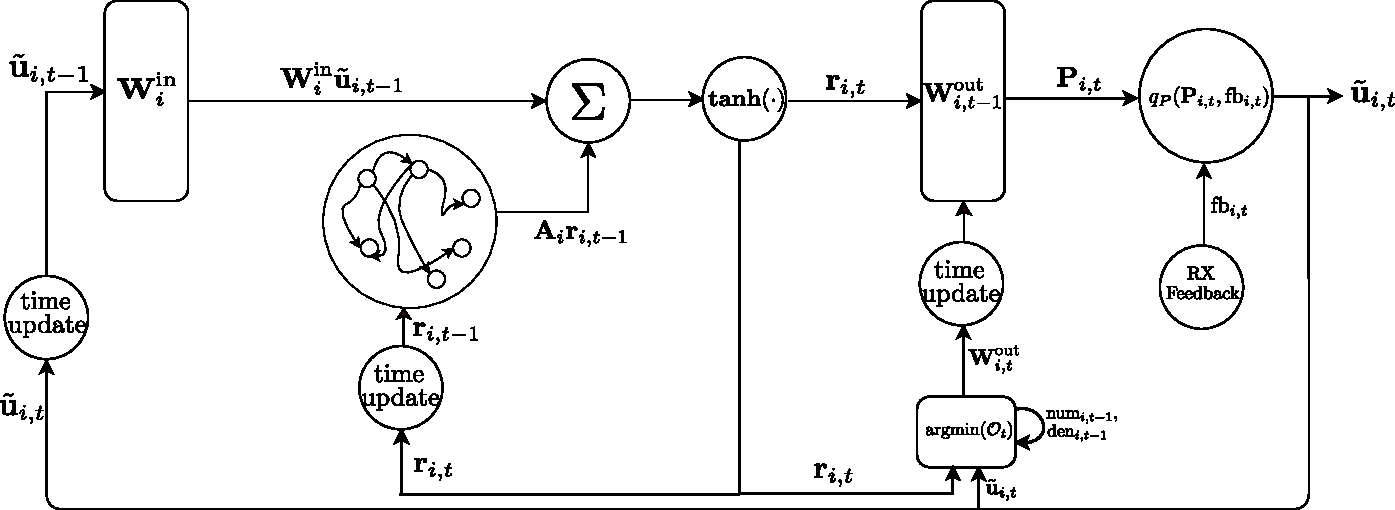
\includegraphics[width=0.8\textwidth]{images/system.pdf}
\label{res_overview}
\caption{An overview of the reservoir computing framework proposed for predictive quantization of $\bu_{i,t}$}
\end{figure*}
$\text{fb}_{i,t}$ is also used to update the spread of the codebooks $T^{\mathcal{C}}_p,T^{\mathcal{C}}_m$.
Depending on whether $\text{fb}_{i,t} \geq 2^{\mathcal{B}-1}$,
i.e. whether the optimum codeword is in $T^{\mathcal{C}}_p$ or
$T^{\mathcal{C}}_m$, the scale parameter $s[k]$, which in turn
controls values of $s_p, s_m$, is updated in the following manner,
$$s_p=g^{\text{min}(s[k-1]+1,0)}, s_m = g^{s[k-1]-1}$$
$$
s[k]=
\begin{cases}
\text{min}(s[k-1]+1,0), \text{ for } \text{fb}_{i,t} \in T^{\mathcal{C}}_p\\
s[k-1]-1, \text{otherwise}\\
\end{cases}
$$
with $s[0]=0$.
Intuitively, the algorithm reduces/increases the spread of the codebook till the operation of reduction/increase is no longer beneficial, i.e. the optimum codeword lies in the higher/lower spread codebook instead.
The scheme used by us to obtain $\text{base}^{\mathcal{C}}$ is similar to the one presented in \cite{Gupt1905:Predictive}, which performs a $k$-means ($k=2^{\mathcal{B}-1}$) clustering on a collection of tangents to obtain an isotropic collection of $2^{\mathcal{B}-1}$ tangent codewords.
This completes the discussion on the quantization function $q_P$ to obtain $\tilde{\bU}_{i,t}=q_P(\bP_{i,t},\text{fb}_{i,t})$ from $\bP_{i,t},\text{fb}_{i,t}$.
%%%%%%%%%%%%%%%%%%%%%%%%%%%%%%%%%%%%%%%%%%%%%%%%%%%%%%%
% More information needed about the adjacency
%%%%%%%%%%%%%%%%%%%%%%%%%%%%%%%%%%%%%%%%%%%%%%%%%%%%%%%
\subsection{Reservoir Training Procedure, the backward pass}
\label{train}
Armed with the descriptions of $f_P, q_P$ we are now ready to describe the training process for the reservoir.
Recall that to obtain $\tilde{\bU}_{i,t}$ from  $\tilde{\bU}_{i,t-1}$, we have,
\begin{equation}
\tilde{\bU}_{i,t}=q_P(\bP_{i,t},\text{fb}_{i,t})=q_P(f_P(\tilde{\bU}_{i,t-1}),\text{fb}_{i,t})
\label{fpqp}
\end{equation}
The key idea here is that as the predicted matrix $\bP_{i,t}$, which is basically the coarse estimate for $\bU_{i,t}$, gets closer to the refined estimate $\tilde{\bU}_{i,t}$, the receiver has to quantize even smaller subspaces and can thus provide an even refined estimate via it's feedback $\text{fb}_{i,t}$.
Hence, for the time instant $t\geq1$, we train the reservoir output coupler such that the following objective function is optimized,
\begin{equation}
\mathcal{O}_t=\sum_{s=1}^{t}\frac{1}{\lambda^{t-s}}||\bp_{i,t}-\tilde{\bu}_{i,t}||^2=\sum_{s=1}^{t}\frac{1}{\lambda^{t-s}}||W_{i,t}^{\text{out}}\br_{i,t}-\tilde{\bu}_{i,t}||^2
\end{equation}
here $\lambda>1$ is the history parameter. We wish to perform the following optimization in order to find the optimum $\bW_{i,t}^{\text{out}}$ from whatever we have observed about $\tilde{\bu}_{i,t}$ uptill now,
\begin{equation}
W_{i,t}^{\text{out}}\gets\text{argmin}_{W_{i,t}^{\text{out}}}(\mathcal{O}_t=\sum_{s=1}^{t}\frac{1}{\lambda^{t-s}}||W_{i,t}^{\text{out}}\br_{i,t}-\tilde{\bu}_{i,t}||^2)
\end{equation}
Computing the gradients $\frac{\partial \mathcal{O}_t}{\partial W_{i,t}^{\text{out}}}$ and setting it to null gives,
\begin{equation}
W_{i,t}^{\text{out}}=\frac{\sum_{s=1}^{t}\frac{1}{\lambda^{t-s}}\texttt{outer}(\tilde{\bu}_{i,s},\br_{i,s})}{\sum_{s=1}^{t}\frac{1}{\lambda^{t-s}}||\br_{i,s}||^2}
\end{equation}
where $\texttt{outer}(\bx,\by)$ is the outer product between $N_x$ dimensional vector $\bx$ and $N_y$ dimensional vector $\by$ to give a $N_x\times N_y$ matrix. Let $\sum_{s=1}^{t}\frac{1}{\lambda^{t-s}}\texttt{outer}(\tilde{\bu}_{i,s},\br_{i,s})$ be $\text{num}_{i,t}$ and $\sum_{s=1}^{t}\frac{1}{\lambda^{t-s}}||\br_{i,s}||^2$ be $\text{den}_{i,t}$, with $W_{i,t}^{\text{out}}=\frac{\text{num}_{i,t}}{\text{den}_{i,t}}$. Observe that,
\begin{equation}
W_{i,t}^{\text{out}}=\frac{\frac{\text{num}_{i,t-1}}{\lambda}+\texttt{outer}(\tilde{\bu}_{i,t},\br_{i,t})}{\frac{\text{den}_{i,t-1}}{\lambda}+||\br_{i,t}||^2}
\label{wout_upd}
\end{equation}
\eqref{wout_upd} makes training of the reservoir easy to implement, and of low complexity as well.
We just need to store the matrix $\text{num}_{i,t-1}$, a number $\text{den}_{i,t-1}$, and using the current reservoir state $\br_{i,t}$ and obtained $\tilde{\bu}_{i,t}$ from \eqref{fpqp}, one can calculate $W_{i,t}^{\text{out}}$ for forward calculation of $\tilde{\bu}_{i,t+1}$.
This completes our technical discussion for the complete reservoir computing based framework for predictive quantization illustrated in Fig. %Ref Fig.
%%%%%%%%%%%%%%%%%%%%%%%%%%%%%%%%%%%%%%%%%%%%%%%%%%%%
%%%%%%%%%%%%%%%%%%%%%%%%%%%%%%%%%%%%%%%%%%%%%%%%%%%%

To conclude this section, now summarize and touch upon the novel points of the reservoir computing based framework proposed for predictive quantization of SVD precoding.
The first key advantage of the proposed framework, over the past work in this line \cite{Gupt1905:Predictive,6891198,6545375} is that the prediction function and quantization function are not independent of each other.
To support the above statement, observe \eqref{res_upd},\eqref{fpqp} to obtain $\bW^{\text{out}}_{i,t}$ from $\tilde{\bu}_{i,t}$, and \eqref{fwd_pred} to obtain $\bP_{i,t+1}$ combinedly,
\begin{equation*}
\highlight{W_{i,t}^{\text{out}}}=\frac{\frac{\text{num}_{i,t-1}}{\lambda}+\texttt{outer}(\highlight{q_P}(f_P(\tilde{\bu}_{i,t-1}),\text{fb}_{i,t}),\br_{i,t})}{\frac{\text{den}_{i,t-1}}{\lambda}+||\br_{i,t}||^2}
\end{equation*}
\begin{equation*}
\highlight{\bP_{i,t+1}}=f_P(\tilde{\bU}_{i,t})=\highlight{\bW^{\text{out}}_{i,t}}\text{tanh}(\bA_i\br_{i,t}+\bW^{\text{in}}_i\highlight{\tilde{\bu}_{i,t}})
\end{equation*}
The dependence between $f_P$ and $q_P$ in our framework is in the sense that the backward pass of the framework ensures that prediction function `'learns' the correlations brought about by $q_P$, in addition to temporal correlations. %Better framing possible
This is done by optimizing $W_{i,t}^{\text{out}}$ such that the prediction output to be as close to the output from $q_P$ (Objective function $\mathcal{O}_t$).
The updated $W_{i,t}^{\text{out}}$ is then used in forward pass to predict $\bP_{i,t+1}$, which is hopefully closer to $\tilde{\bU}_{i,t+1}$ than $\bP_{i,t}$ was to $\tilde{\bU}_{i,t}$ due to optimization of $\mathcal{O}_t$.

The second key advantage of the proposed scheme comes from the ease of training the reservoir, entailed by \eqref{res_upd}.
By storing just one matrix $\text{num}_{i,t}$ and a number $\text{den}_{i,t}$, we can capture the enitre history of the precoding matrices, with past values weighted by $\lambda$.
This is a departure from previous schemes \cite{Gupt1905:Predictive,6891198,6545375} which store the past $n$ (which has to be pre-decided) precoders in a $n$ sized cyclic buffer kind-of arrangement.
Reservoir computing, thus proposes an easier to implement data centric scheme, which is a rarity for typical data centric ML based schemes.


\section{Simulation Results}
\label{section4}
\subsection{Simulation setting considered}
\label{setting}
\noindent We compare the results of the proposed reservoir computing framework with the predictive quantization scheme presented in \cite{6891198}, which also captures the temporal correlations to enable reduced quantization error.
\subsection{Quantization Error, BER and Achievable Rate Results}
\label{res}
%Qtisn error with 1000 chan evols
%Qtisn error with 100 chan evols
%BER
%Achievable rat
\section{Conclusions and Future Work}
\label{section5}


% \section{Acknowledgment}
% % \label {section6}
% % \input{sections/6_section.tex}
% Parts of this work was supported by the Bharti Centre for Communication in
% IIT Bombay, and the Visvesvaraya
% PhD Scheme of Ministry of Electronics \& Information Technology,
% Government of India, being implemented by Digital India Corporation.


\renewcommand{\bibfont}{\footnotesize}
\bibliography{IEEEabrv,main}
\bibliographystyle{IEEEtran}
\end{document}

% Remove the first para of FSM. State what r1,r2,d,\theta are in the FSM model states themselves. As a concluding statement of STAT-2 state that using the
% inherit geometery of the problem, we get AoA
